%%%%%%%%%%%%%%%%%%%%%%%%%%%%%%%%%%%%%%%%%
% Beamer Presentation
% LaTeX Template
% Version 1.0 (10/11/12)
%
% This template has been downloaded from:
% http://www.LaTeXTemplates.com
%
% License:
% CC BY-NC-SA 3.0 (http://creativecommons.org/licenses/by-nc-sa/3.0/)
%
%%%%%%%%%%%%%%%%%%%%%%%%%%%%%%%%%%%%%%%%%

%----------------------------------------------------------------------------------------
%	PACKAGES AND THEMES
%----------------------------------------------------------------------------------------

\documentclass{beamer}

\mode<presentation> {

% The Beamer class comes with a number of default slide themes
% which change the colors and layouts of slides. Below this is a list
% of all the themes, uncomment each in turn to see what they look like.

%\usetheme{default}
%\usetheme{AnnArbor}
%\usetheme{Antibes}
%\usetheme{Bergen}
%\usetheme{Berkeley}
%\usetheme{Berlin}
%\usetheme{Boadilla}
%\usetheme{CambridgeUS}
%\usetheme{Copenhagen}
%\usetheme{Darmstadt}
%\usetheme{Dresden}
%\usetheme{Frankfurt}
%\usetheme{Goettingen}
%\usetheme{Hannover}
%\usetheme{Ilmenau}
%\usetheme{JuanLesPins}
%\usetheme{Luebeck}
\usetheme{Madrid}
%\usetheme{Malmoe}
%\usetheme{Marburg}
%\usetheme{Montpellier}
%\usetheme{PaloAlto}
%\usetheme{Pittsburgh}
%\usetheme{Rochester}
%\usetheme{Singapore}
%\usetheme{Szeged}
%\usetheme{Warsaw}

% As well as themes, the Beamer class has a number of color themes
% for any slide theme. Uncomment each of these in turn to see how it
% changes the colors of your current slide theme.

%\usecolortheme{albatross}
%\usecolortheme{beaver}
%\usecolortheme{beetle}
%\usecolortheme{crane}
%\usecolortheme{dolphin}
%\usecolortheme{dove}
%\usecolortheme{fly}
%\usecolortheme{lily}
\usecolortheme{orchid}
%\usecolortheme{rose}
%\usecolortheme{seagull}
%\usecolortheme{seahorse}
%\usecolortheme{whale}
%\usecolortheme{wolverine}

%\setbeamertemplate{footline} % To remove the footer line in all slides uncomment this line
%\setbeamertemplate{footline}[page number] % To replace the footer line in all slides with a simple slide count uncomment this line

%\setbeamertemplate{navigation symbols}{} % To remove the navigation symbols from the bottom of all slides uncomment this line
}

\usepackage{graphicx} % Allows including images
\usepackage{booktabs} % Allows the use of \toprule, \midrule and \bottomrule in tables

%----------------------------------------------------------------------------------------
%	TITLE PAGE
%----------------------------------------------------------------------------------------

\title[Isoprene in the Southern Ocean]{Ecological modeling of isoprene in the Southern Ocean} % The short title appears at the bottom of every slide, the full title is only on the title page

\author{Pablo Rodriguez-Ros} % Your name
\institute[ICM-CSIC] % Your institution as it will appear on the bottom of every slide, may be shorthand to save space
{
Institute of Marine Sciences (ICM) -- Spanish National Research Council (CSIC) \\ \bigskip \textbf{SORPASSO Project (ACE 8) \\ NOSASSO -- Plymouth Marine Laboratory (PML)}\\ % Your institution for the title page

\medskip
P. Rodr\'{i}guez-Ros, C. Nissen, P. Cort\'{e}s , N. Gruber, R. Sim\'{o}, S. Vallina, M. Vogt

\medskip

\textit{pros@icm.csic.es\\Twitter: @pablorros\_\\} % Your email address
}

\titlegraphic{
\includegraphics[width=4cm]{icm-logo.jpg}\hspace*{0.5cm}~%

\includegraphics[width=3cm]{image_imageformat_lightbox_404647511.jpg}\hspace*{0.5cm}~%

\includegraphics[width=1.5cm]{declaracion_IEO_prensa_gallega.jpg}\hspace*{0.5cm}~%

\includegraphics[width=1.5cm]{ace.png}%
}

\begin{document}

\begin{frame}
\titlepage % Print the title page as the first slide
\date{\today} % Date, can be changed to a custom date
\end{frame}

\begin{frame}
\frametitle{Overview} % Table of contents slide, comment this block out to remove it
\tableofcontents % Throughout your presentation, if you choose to use \section{} and \subsection{} commands, these will automatically be printed on this slide as an overview of your presentation
\end{frame}

%----------------------------------------------------------------------------------------
%	PRESENTATION SLIDES
%----------------------------------------------------------------------------------------

%------------------------------------------------
\section{Isoprene: the basics} 

\begin{frame}
\frametitle{Isoprene: basics}

\begin{itemize}
\item On land: Photosynthetic vegetation, \textbf{400-500 Tg C yr -1} (Guenther, 1995; Mulller, 2008)
\item On the oceans: marine microbiota \textbf{0.21-11.6 Tg C yr -1} (Booge et al, 2016; Luo et al, 2010). \textbf{Still strong discrepancies!}

\end{itemize}

\begin{figure}
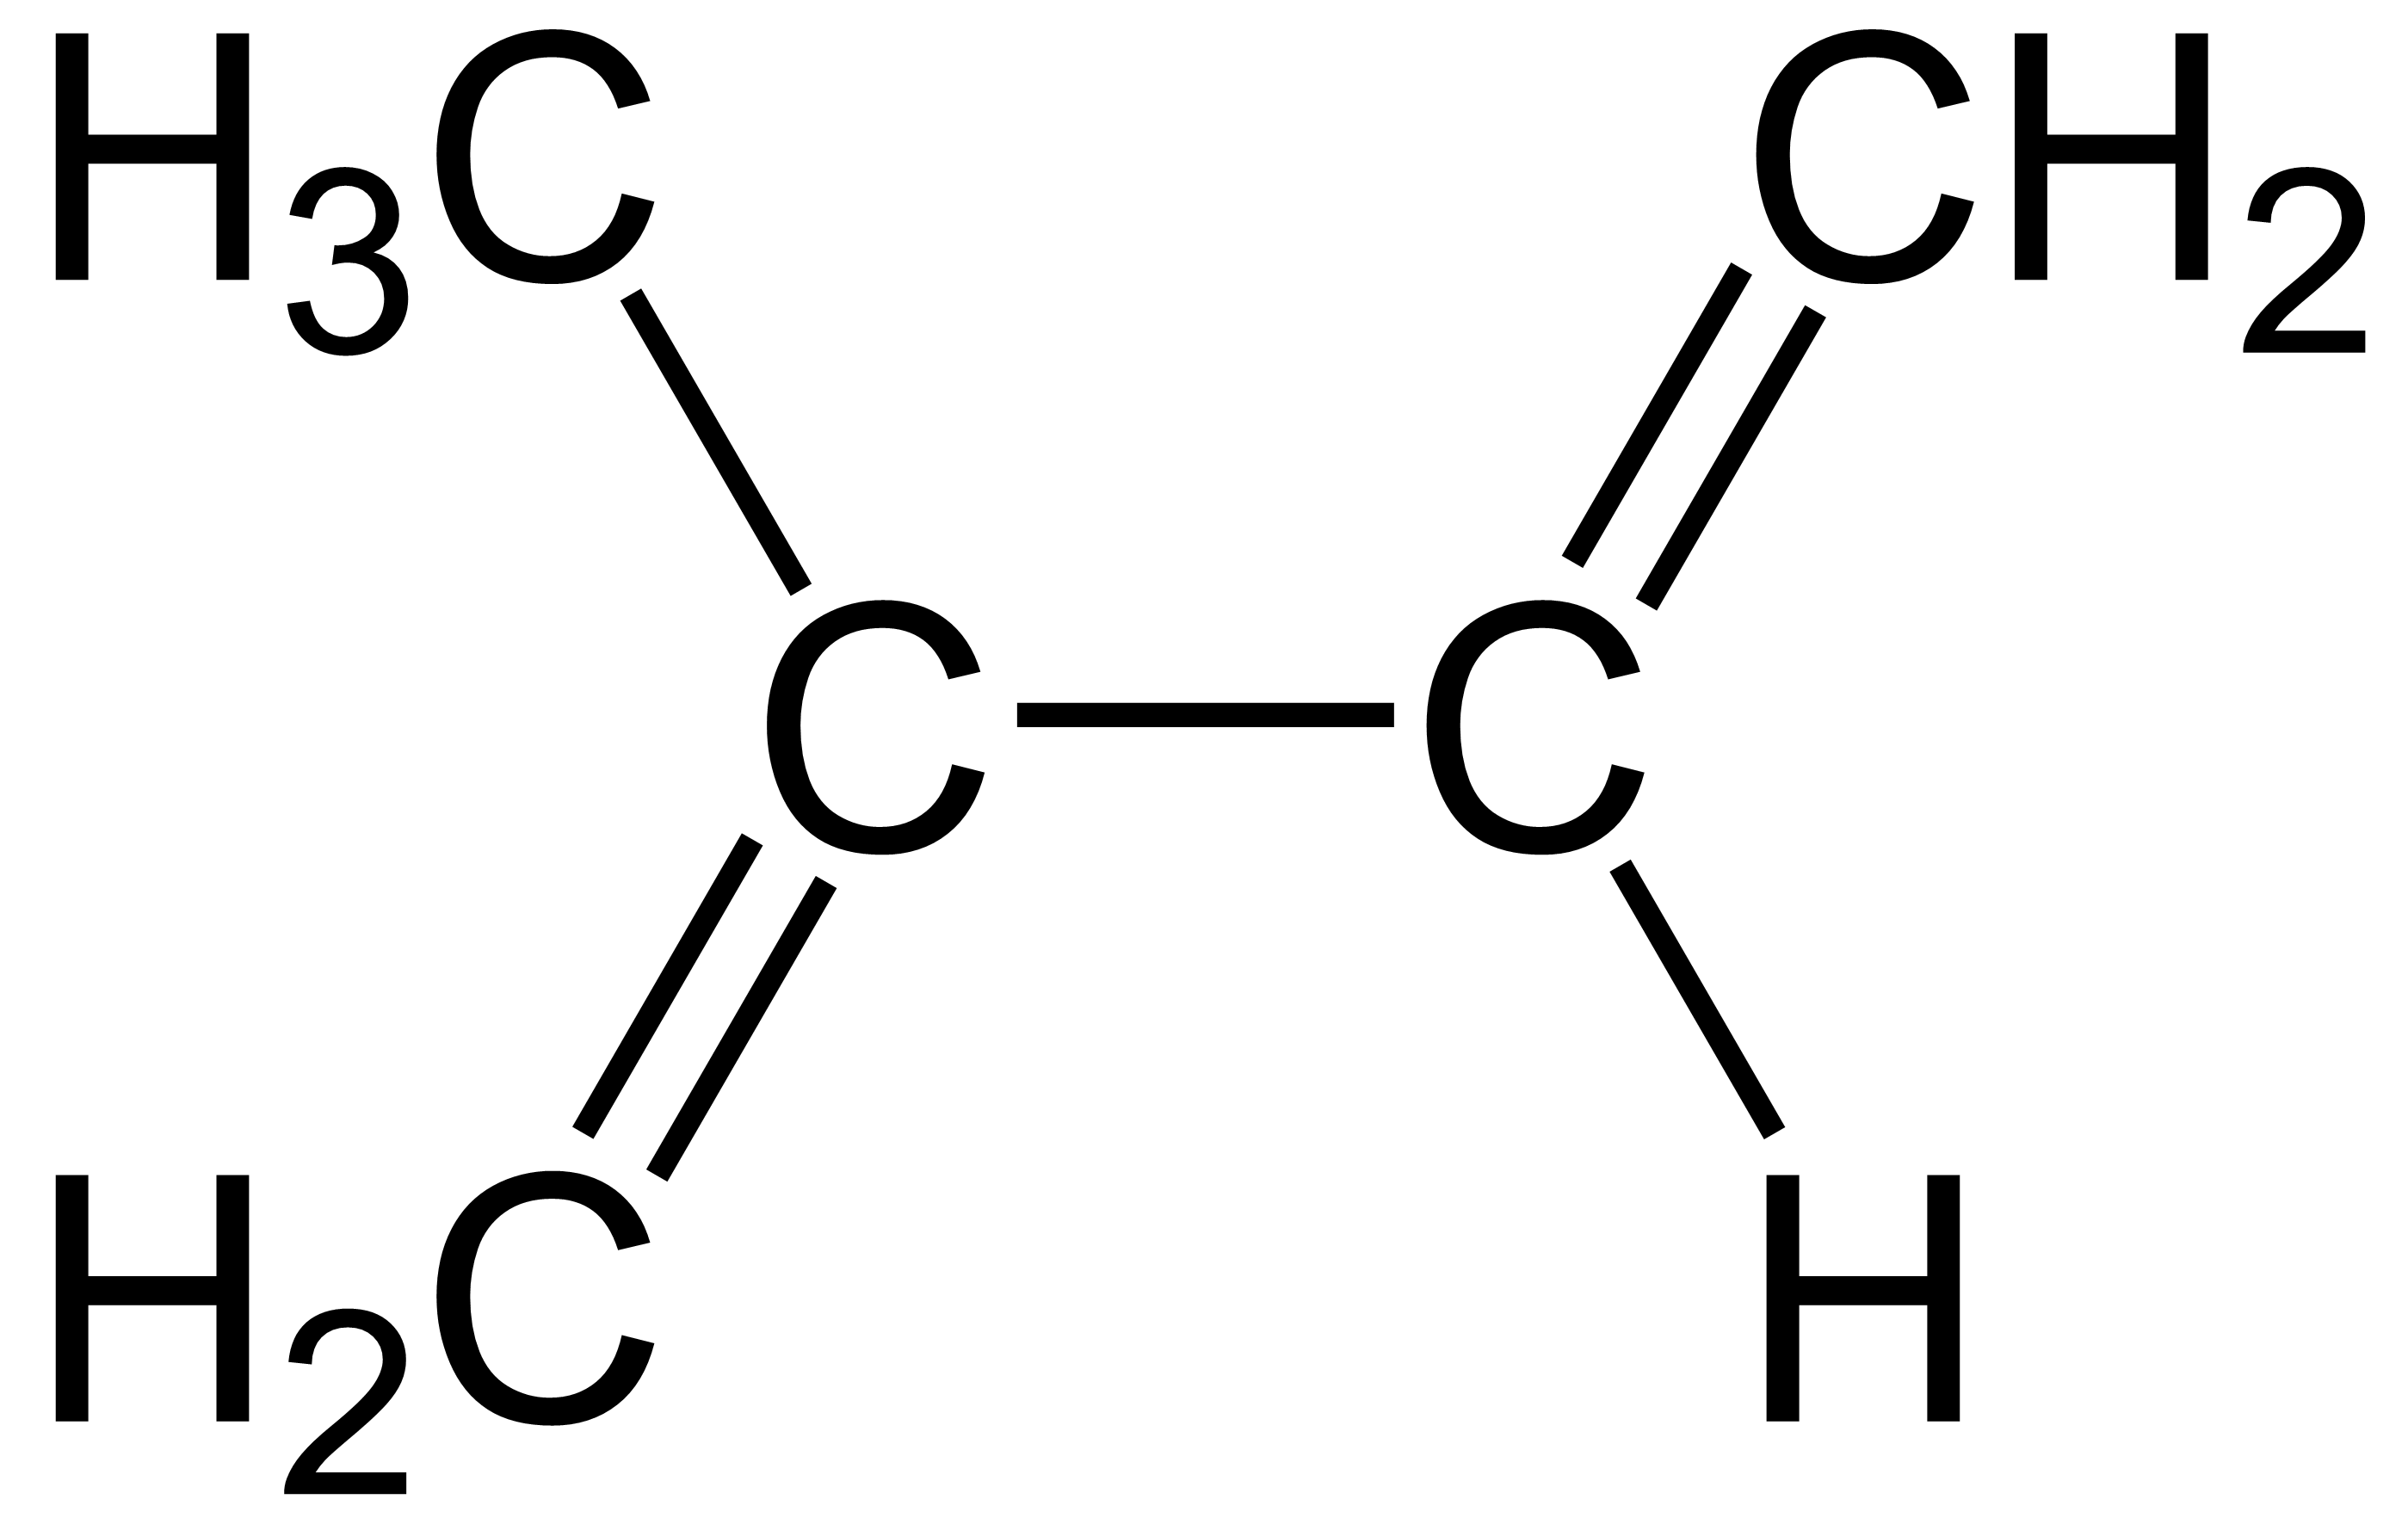
\includegraphics[width=0.5\linewidth]{Isoprene-Structure.png}
\end{figure}

\end{frame}

%------------------------------------------------

\begin{frame}
\frametitle{SOLAS Theme 4}
Interconnections between aerosols, clouds, and marine ecosystems.
\begin{figure}
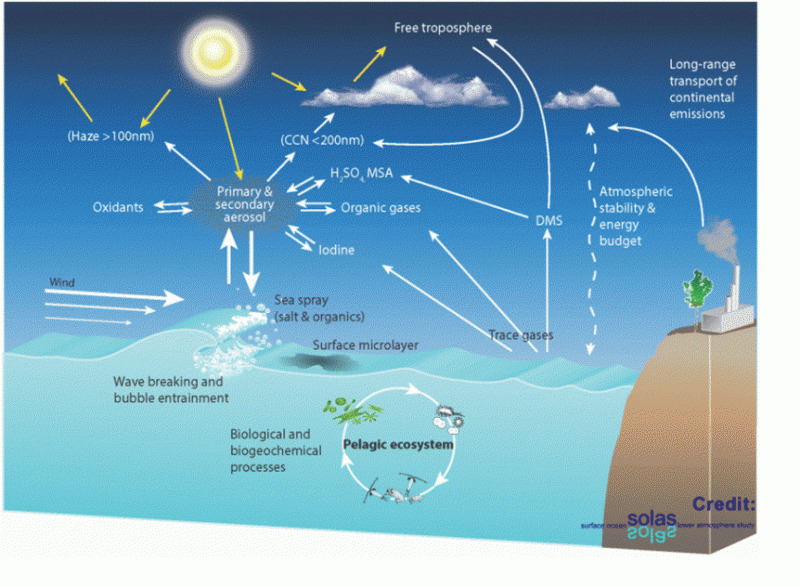
\includegraphics[width=0.8\linewidth]{theme4.jpg}
\end{figure}
\end{frame}


%\subsection{Booge et al. 2016 compilation}
\section{Isoprene in ROMS-BEC model: approach and results}

\begin{frame}
\frametitle{ROMS-BEC Model - ETH, Zurich}
- UP (Environmental Systems Group). PI: Nicolas Gruber.\\
- Collaboration with Cara Nissen and Dr. Meike Vogt.\\
\bigskip
\textbf{ROMS}: Physical model - Regional: Southern Ocean \textbf{($<$ 30S !)}.\\
\textbf{BEC}: Biogeochemical -- Ecological model.
\begin{figure}
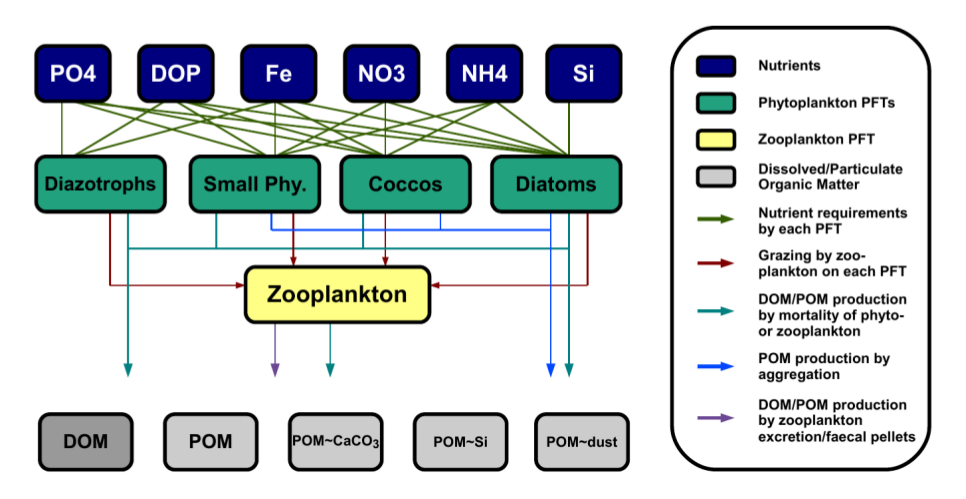
\includegraphics[width=0.9\linewidth]{Screenshot_from_2016-11-16_18_37_12.png}
\end{figure}

\end{frame}

%%%%%%%%%%%55

\begin{frame}
\frametitle{Isoprene production model \\ Based on Palmer and Shaw, 1995; and Booge et al. 2016.}
\begin{center}
\scalebox{1.5}{
$\frac{\mathrm{d \, ISO}}{\mathrm{dt}} = \mathrm{P}_{\mathrm{PFT}} - \mathrm{L}_{\mathrm{BIO}} - \mathrm{L}_{\mathrm{CHEM}} - \mathrm{L}_{\mathrm{ATM}}$} \\

\bigskip
\textbf{Sources}\\
\bigskip

\textbf{Isoprene production:} $\mathrm{P}_{\mathrm{PFT}} = \sum^{3}_{i=1}\rho^{i}_{chl} \cdot [PFT^{i}_{chl}]$\\
\bigskip

\textbf{Sinks}\\
\bigskip

\textbf{Biological loss rates:} $\mathrm{L}_{\mathrm{BIO}} = [Iso]_{w} \cdot K_{BIOL}$\\
\bigskip

\textbf{Chemical loss rates:} $\mathrm{L}_{\mathrm{CHEM}} = [Iso]_{w} \cdot K_{CHEM}$\\
\bigskip

 \textbf{Ocean-atmosphere flux:} $\mathrm{L}_{\mathrm{ATM}} = [Iso]_{w} \cdot K_{AS}$

\end{center}
\tiny  Rodriguez-Ros, Nissen, et al (In preparation).

\end{frame}

%%%%%%%%%%%%%%%%%%%%%%%%%%%%%%%%%%%

\begin{frame}
\frametitle{Iso ROMS-BEC set up}

\begin{center}


\begin{table}[h!]
\centering
\scalebox{1.5}{
$\frac{\mathrm{d \, Iso}}{\mathrm{dt}} = \mathrm{P}_{\mathrm{PFT}} - \mathrm{L}_{\mathrm{BIO}} - \mathrm{L}_{\mathrm{CHEM}} - \mathrm{L}_{\mathrm{ATM}}$} \\

\bigskip
\caption{Isoprene model parameters from Booge et al, 2016.}

\begin{tabular}[ht]{ c|c|c|c|c|c } 

 \textbf{Parameter} & \textbf{Unit} &  \textbf{Value} & \textbf{Variability} \\\hline

 $\rho^{\mathrm{Diat}}_{\mathrm{chl}}$     & $\mathrm{mmol} \; \mathrm{mgChl}^{\mathrm{-1}} \; \mathrm{d}^{\mathrm{-1}}$  & 2.06 & 0.56 - 9.36 \\

$\rho^{\mathrm{Cocco}}_{\mathrm{chl}}$     & $\mathrm{mmol} \; \mathrm{mgChl}^{\mathrm{-1}} \; \mathrm{d}^{\mathrm{-1}}$  & 5.54 & 1 - 11.28 \\

$\rho^{\mathrm{SP}}_{\mathrm{chl}}$     & $\mathrm{mmol} \; \mathrm{mgChl}^{\mathrm{-1}} \; \mathrm{d}^{\mathrm{-1}}$  & 5.73 & 1.4 - 12.4\\

$\mathrm{L}_{\mathrm{Bio}}$ & $\mathrm{d}^{\mathrm{-1}}$ & 0.06 & 0 - 0.06 \\

$\mathrm{k}_{\mathrm{OH}} \cdot \mathrm{C}_{\mathrm{OH}}$ & $\mathrm{d}^{\mathrm{-1}}$ & 0.0518 & - \\

$\mathrm{k}_{\mathrm{O_{\mathrm{2}}}} \cdot \mathrm{C}_{\mathrm{O_{\mathrm{2}}}}$ & $\mathrm{d}^{\mathrm{-1}}$  & 0.0009 & -  \\

\end{tabular}

\end{table}

\end{center}
\tiny  Rodriguez-Ros, Nissen, et al (In preparation).

\end{frame}

%\subsection{Total emission}
%\subsection{Seasonal pattern}
%\subsection{Depth distribution}
%\subsection{Validation}
%\subsection{Comparison to other global estimate
%\subsection{PEGASO in situ rates}


%------------------------------------------------

\begin{frame}
\frametitle{Accumulated Isoprene emission (1-year) in ROMS-BEC}
- Maximum concentration around \textbf{200 pM}, average \textbf{20-40 pM}.
\begin{figure}
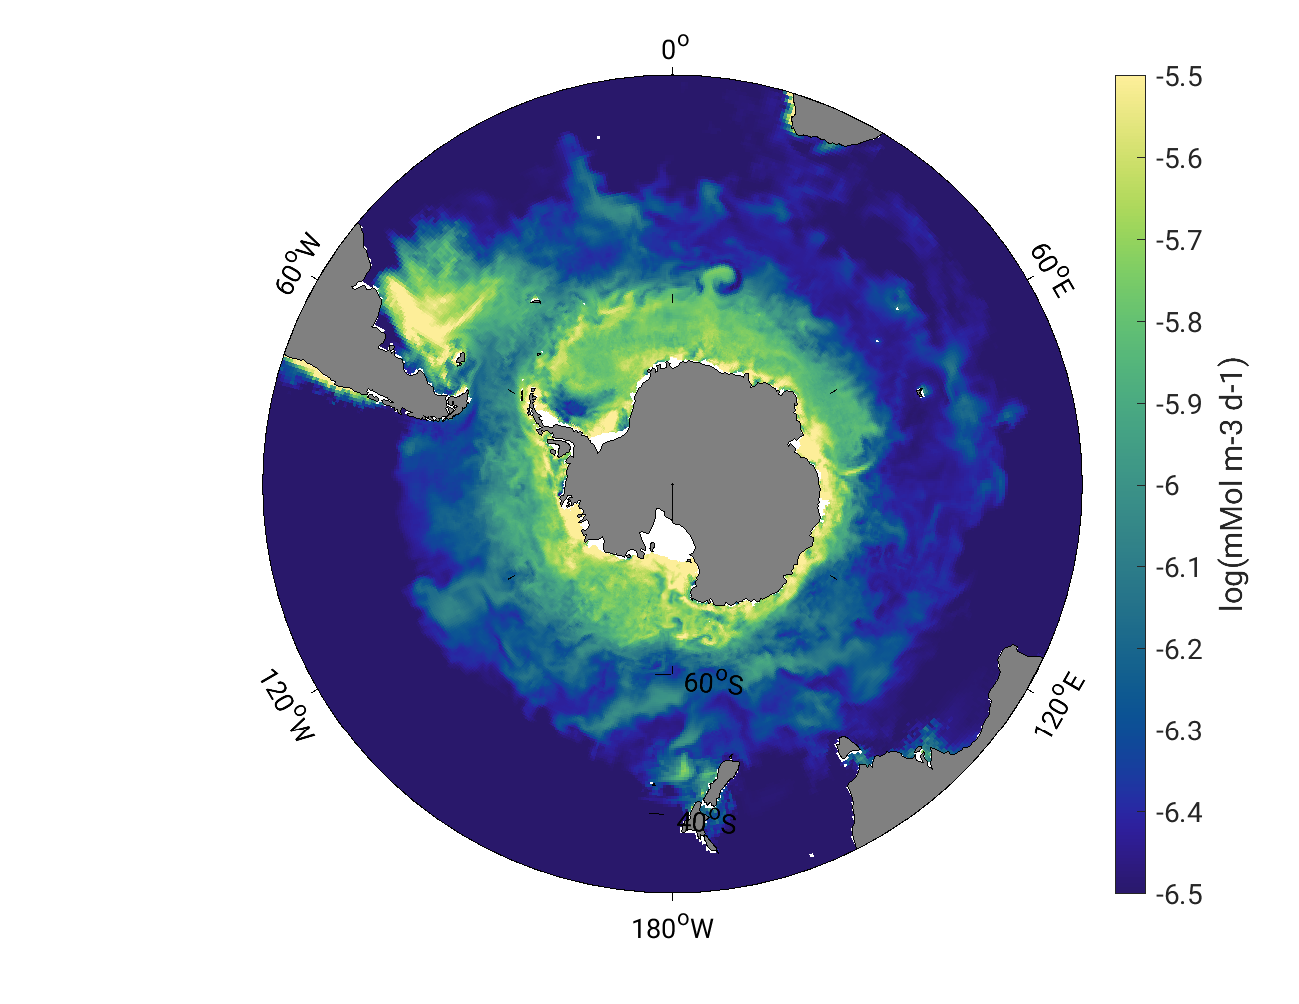
\includegraphics[width=0.70\linewidth]{ISO_PROD_annual_at_10m_031.png}
\end{figure}
\tiny  Rodriguez-Ros, Nissen, et al (In preparation).
\end{frame}

%------------------------------------------------

\begin{frame}
\frametitle{Seasonality of Isoprene emissions in ROMS-BEC}
- Higher emissions in \textbf{summer} period.
\begin{figure}
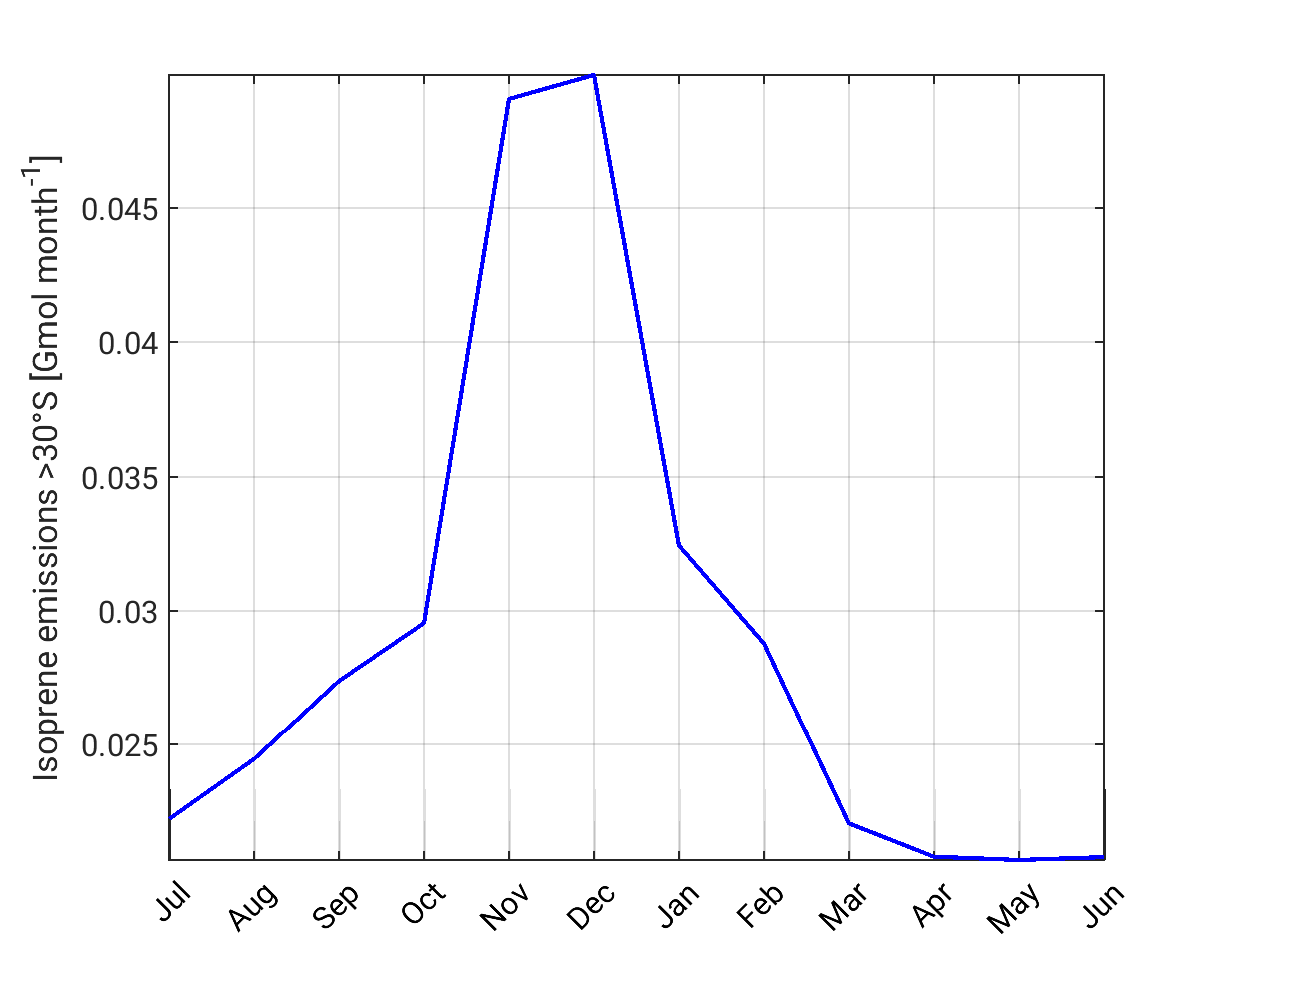
\includegraphics[width=0.70\linewidth]{Isoprene_emissions_monthly_timeSeries_031.png}
\end{figure}
\tiny  Rodriguez-Ros, Nissen, et al (In preparation).
\end{frame}

%%%%%%%%%%%%%%%%%%%%%%%%%%%
\begin{frame}
\frametitle{Hovmoller diagram of isoprene surface (5m) production and emission in ROMS-BEC.}
\begin{figure}
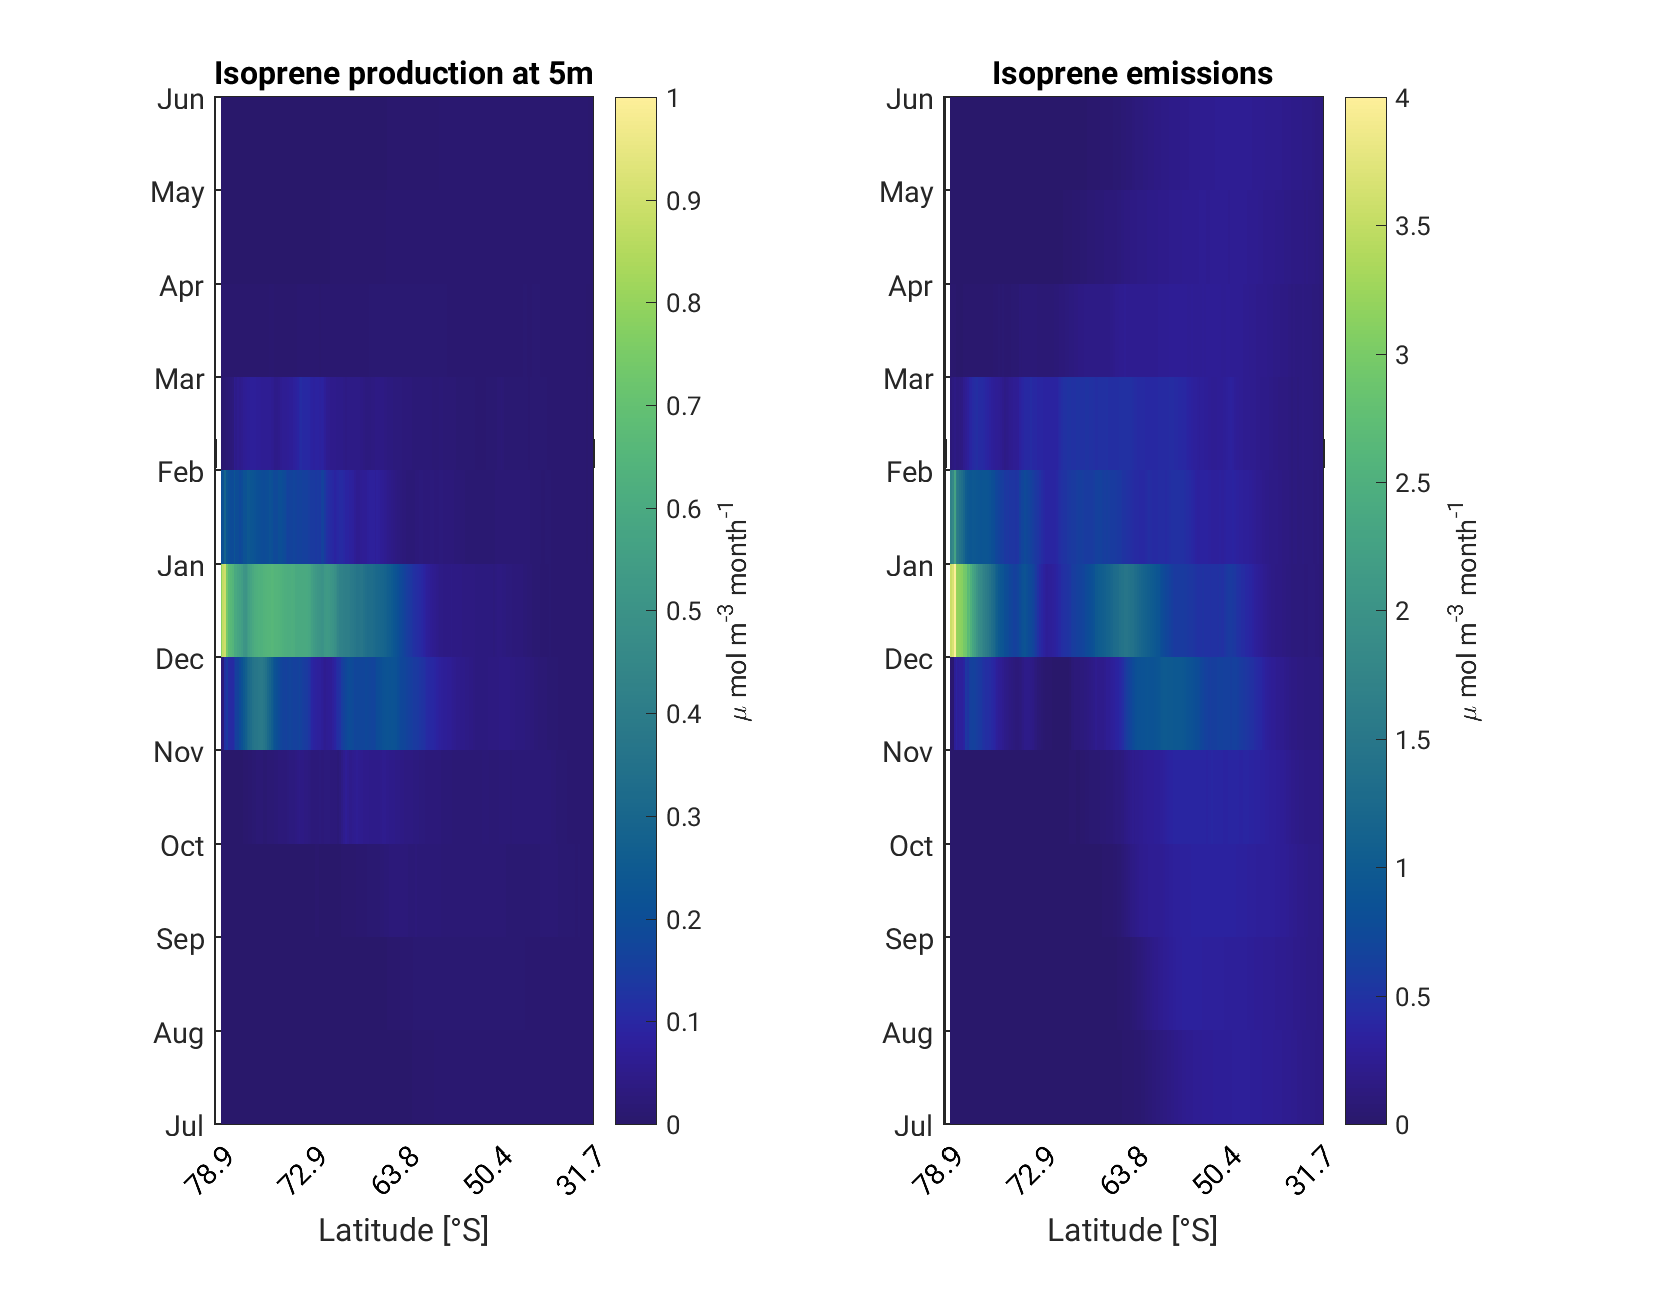
\includegraphics[width=0.7\linewidth]{Hovmoller_031_isoprene_prod_at_5m_srf_flux_circumpolar.png}
\end{figure}
\tiny  Rodriguez-Ros, Nissen, et al (In preparation).

\end{frame}

%------------------------------------------------

\begin{frame}
\frametitle{Global vs Southern Ocean estimates}

\begin{center}

\begin{table}[h!]

\centering

\caption{Global estimates of isoprene emissions for the Global Ocean in comparison with our preliminary results for the Southern Ocean [Rodriguez-Ros et al., 2018, in preparation]. A more updated verssion can be found in Bruggemannet al 2018.}

\label{tab:global}

\begin{tabular}[ht]{ c|c|c|c|c|c } 

\textbf{Area} & \textbf{Reference} & \textbf{Range*} & \textbf{Approach} \\\hline

S. O. & ISO.ROMS.BEC & \textbf{0.29}  & 	 Bottom-up  \\
G. O. & Palmer et al, 2015  & 0.1   & Top-down \\
G. O. & Booge et al, 2016 & 0.21 &   Bottom-up\\
G. O. & Arnold et al, 2009 & 0.31 - 1.9 &  Bottom-up -- Top-down \\
G. O.  & Luo et al, 2010 & 0.32 - 11.6  &  Bottom-up -- Top-down \\
G. O.  & Gantt et al, 2009 & 1.9 &  Bottom-up\\
G. O.  & Bruggemann et al, 2018 & 0.70 - 1.52 & Bottom-up  \\
G. O.  & Shaw et al, 2010 & 0.085 - 11.6 & Bottom-up -- Top-down \\
\end{tabular}
\bigskip
* \textbf{Units}:  Tg C yr -1 

\end{table}

\end{center}
\tiny  Rodriguez-Ros, Nissen, et al (In preparation).

\end{frame}
%------------------------------------------------
\section{Validation: Isoprene Southern Ocean database}
\begin{frame}
\frametitle{Validation}
TransPEGASO + ACE Leg 0
\begin{figure}
\includegraphics[width=0.6\linewidth]{tpeg_ace4.png}
\end{figure}
\end{frame}

\begin{frame}
\frametitle{Validation}
PEGASO Cruise
\begin{figure}
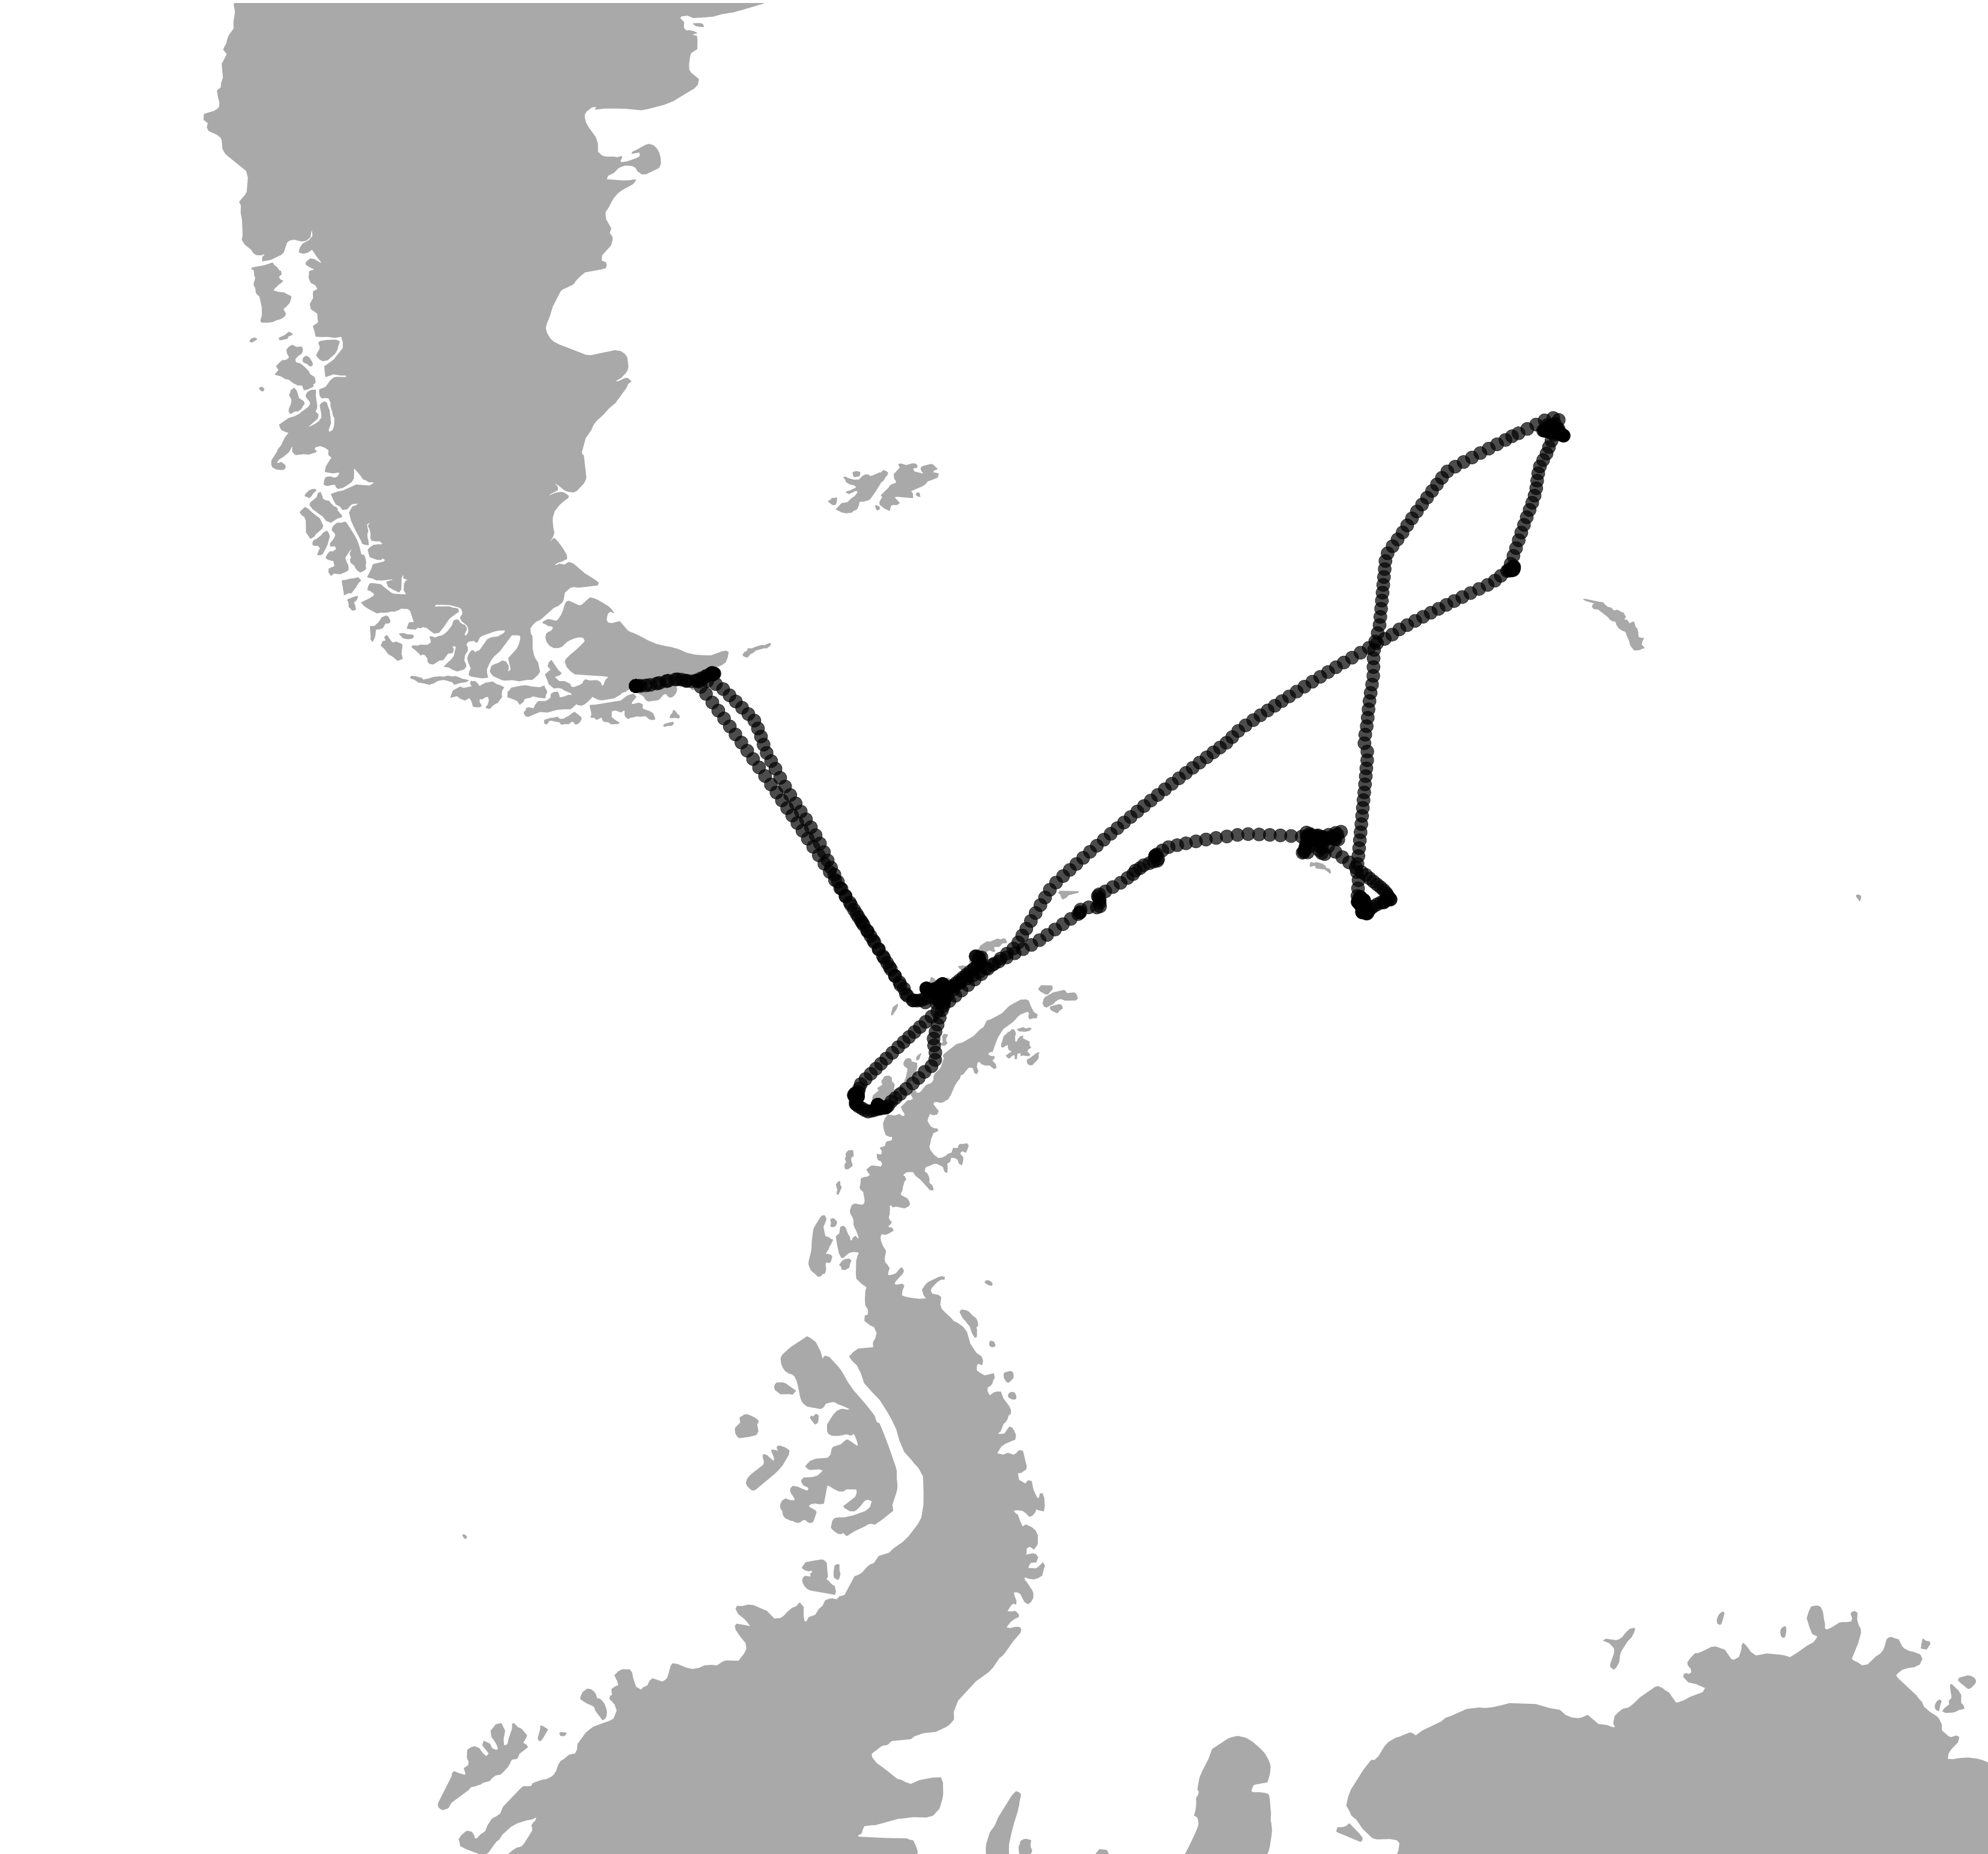
\includegraphics[width=0.6\linewidth]{peg.png}
\end{figure}
\end{frame}

\begin{frame}
\frametitle{Validation}
ACE Expedition
\begin{figure}
\includegraphics[width=0.6\linewidth]{acea.png}
\end{figure}
\end{frame}

\begin{frame}
\frametitle{Validation}
\textbf{Isoprene antarctic dataset}: TransPEGASO + PEGASO + ACE.\\
- \textbf{Around 400 hundred data-points!}
\begin{figure}
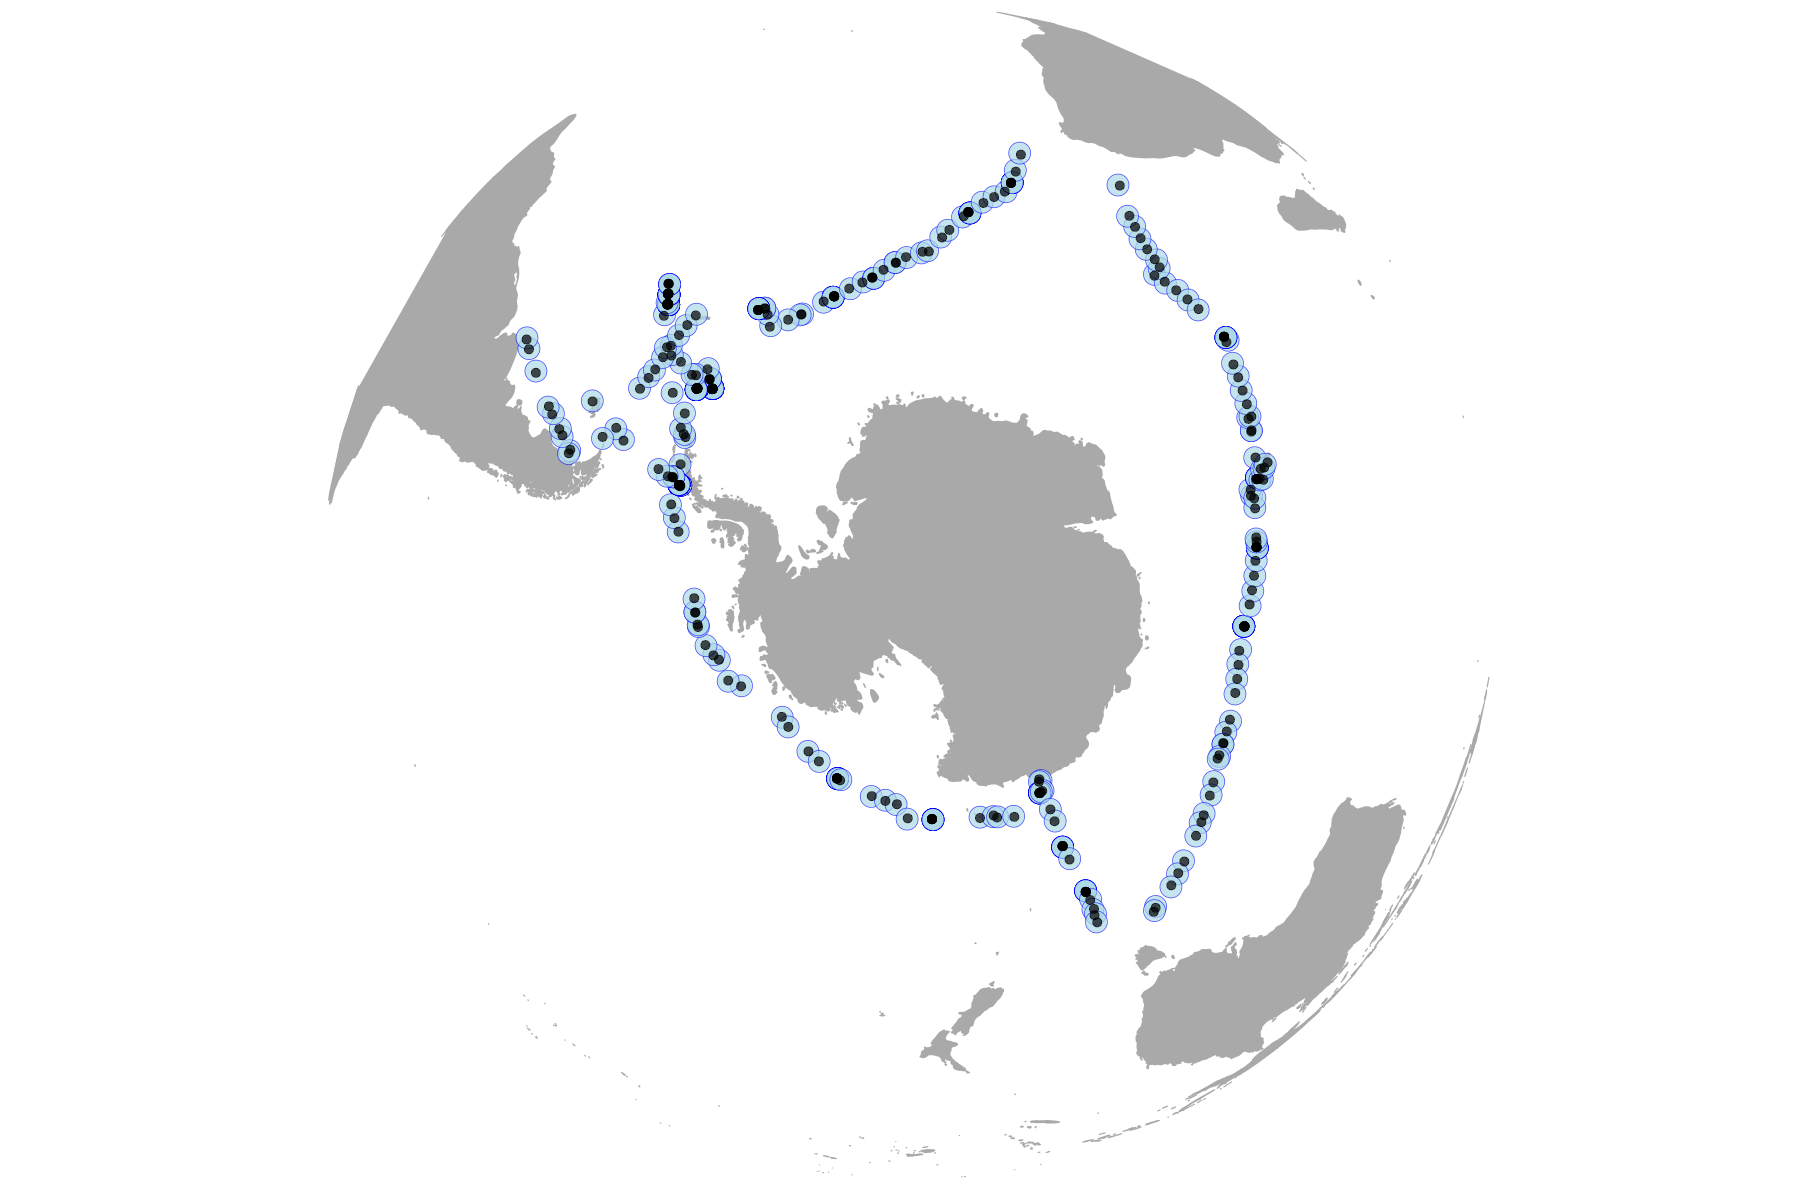
\includegraphics[width=0.9\linewidth]{validation_isoprene_roms_bec_ant.png}
\end{figure}
\end{frame}

\begin{frame}
\frametitle{Validation}
\textbf{Isoprene concentration - R (pearsons) = 0.44}

\begin{figure}
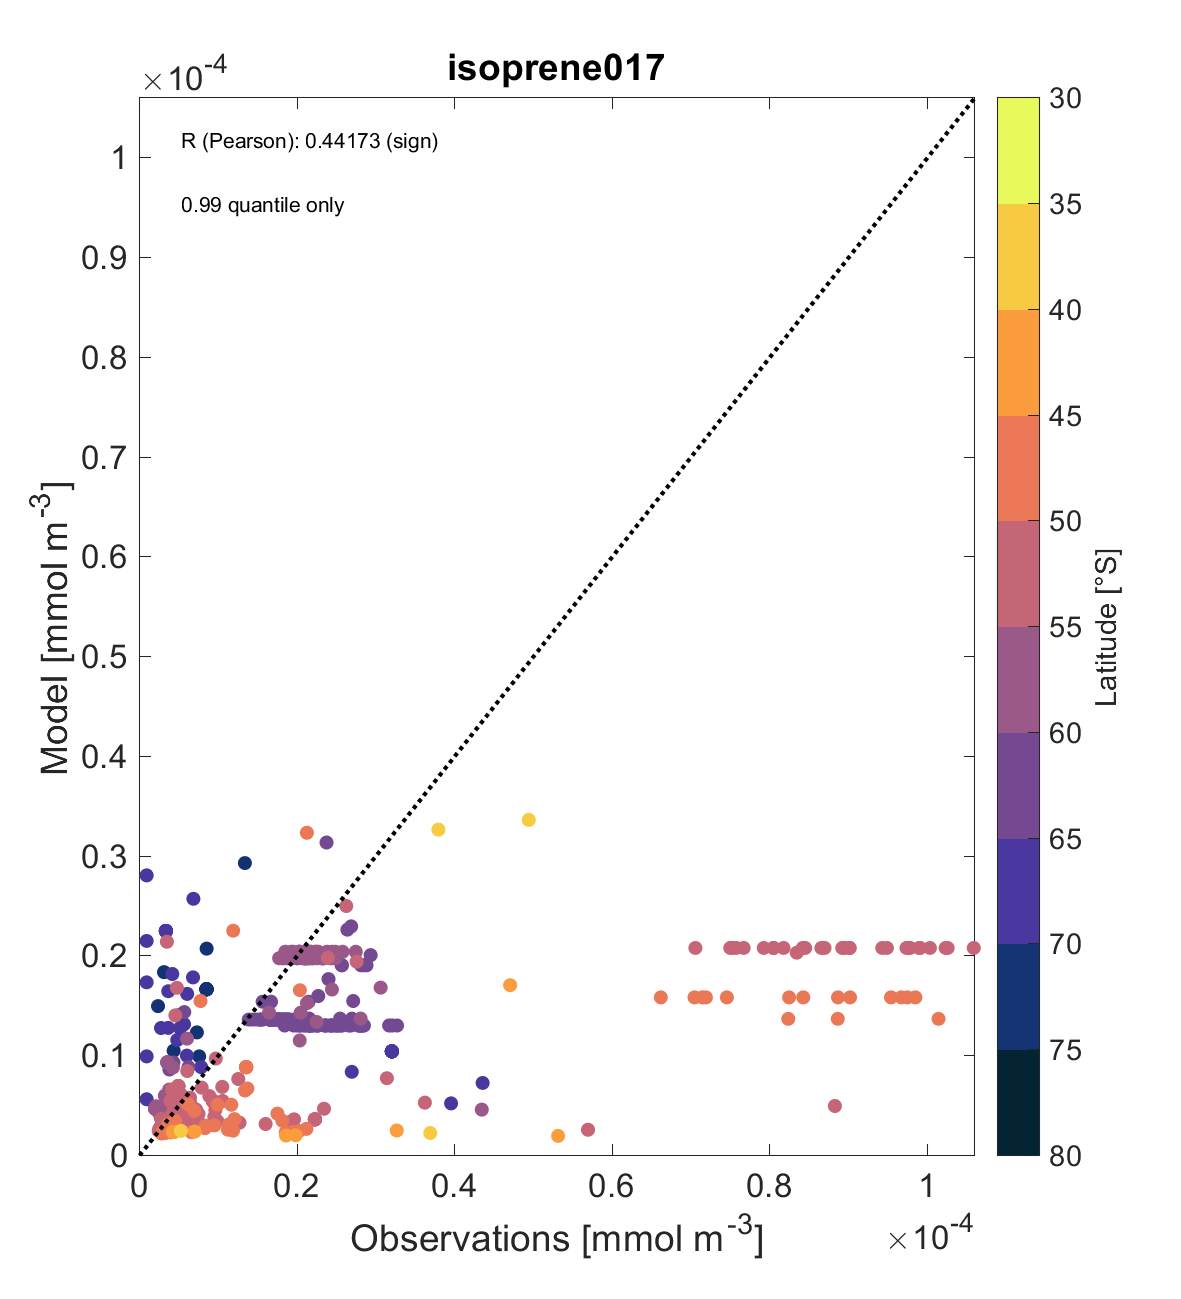
\includegraphics[width=0.50\linewidth]{isoprene_observations_vs_modelo_017_3080_2_Lat_099_PAPER.png}
\end{figure}
\tiny  Rodriguez-Ros, Nissen, et al (In preparation).
\end{frame}

\section{}

\begin{frame}
\frametitle{New PFT's rates from in situ data}
- PEGASO cruise: In situ production rates.
\begin{center}
\scalebox{1.2}{
$\frac{ΔIso_{w}}{d} =  P - \overline{Iso}_{w} \cdot (Σ k_{CHEM, i} C_{xi}) - \overline{Iso}_{w}  \cdot k_{BIOL} - \frac{F_{Iso}}{MLD} - L_{MIX}$ }

\bigskip

\scalebox{1.2}{
$P_{chla} = \frac{P}{chla}$}
\end{center}
\begin{center}
\begin{table}[b!]
\caption{Isoprene production PFT rates on every bloom.}
\centering
\begin{tabular}[ht]{ c|c|c|c|c|c } 

 \textbf{Bloom} & \textbf{Area} & \textbf{ $\mathrm{P_{chla}}$* }& \textbf{Dominant PFT(s)} \\\hline
 I &  Orkney Islands & 3.32   & 26\% hapto., 37\% crypto.  \\
II &   Weddell Sea&  11.06   &  80\% hapto.\\
 III &  S. Georgia Islands & 4.12 & 80\% diatoms  \\
 IV & Gerlache Strait & 1.77  &  57\% crypto., 24\% hapto.\\
\end{tabular}
\end{table}
\bigskip
* \textbf{Units}:  $\mathrm{mmol} \; \mathrm{mgChl}^{\mathrm{-1}} \; \mathrm{d}^{\mathrm{-1}}$  .
\end{center}
\end{frame}

\section{What is next?}

\begin{frame}
\frametitle{Isoprene ACE dataset - What is next?}

%------------------------------------------------
\begin{itemize}
\item \textbf{Remote sensing} approach to detect isoprene concentration in the Southern Ocean. Also testing the DMS algorithm developed by \textbf{Gali et al. 2018}.
\item To develop \textbf{statistical algorithms} of isoprene based on its relationship with pigments and environmental variables.
\item To explore the coupled behavior of\textbf{ isoprene/DMS in seawater and the atmosphere} along ACE Expedition -\textbf{ J. Schmale} (PSI, Switzerland).
\item To compile datasets from the Southern Ocean from different works: Ooki et al, 2015; Booge et al, 2016; Hackemberg et al, 2017. \textbf{Improve the validation of ROMS-BEC model outputs!}
\end{itemize}
%------------------------------------------------
\end{frame}
%------------------------------------------------
\section{Some useful bibliography}
\begin{frame}
\frametitle{Some useful bibliography ...}
\footnotesize{
\begin{thebibliography}{99} % Beamer does not support BibTeX so references must be inserted manually as below
 
\bibitem[arnold2009]{p1} Arnold et al (2009)
\newblock Evaluation of the global oceanic isoprene source and its impacts on marine organic carbon aerosol

\bibitem[booge2016]{p1} Booge et al (2016)
\newblock Can simple models predict large-scale surface ocean isoprene concentrations?

\bibitem[hackemberg2017]{p1} Hackemberg et al (2017)
\newblock Potential controls of isoprene in the surface ocean

\bibitem[nissenatal2018]{p1} Nissen et al. 2018 (Under review)
\newblock Factors controlling coccolithophore biogeography in the Southern Ocean\\

--------------------------------------------------------------------------

\bibitem[carpenter2011]{p1} Carpenter et al (2011)
\newblock Ocean-atmosphere trace gas exchange

\bibitem[SOLAS2014]{p1} P. S. Liss et al. (2014)
\newblock  "SOLAS Book" - Ocean-Atmosphere Interactions of Gases and Particles

\end{thebibliography}
}
\end{frame}

%------------------------------------------------

\begin{frame}
\Huge{\centerline{Thank you!}}
\begin{figure}
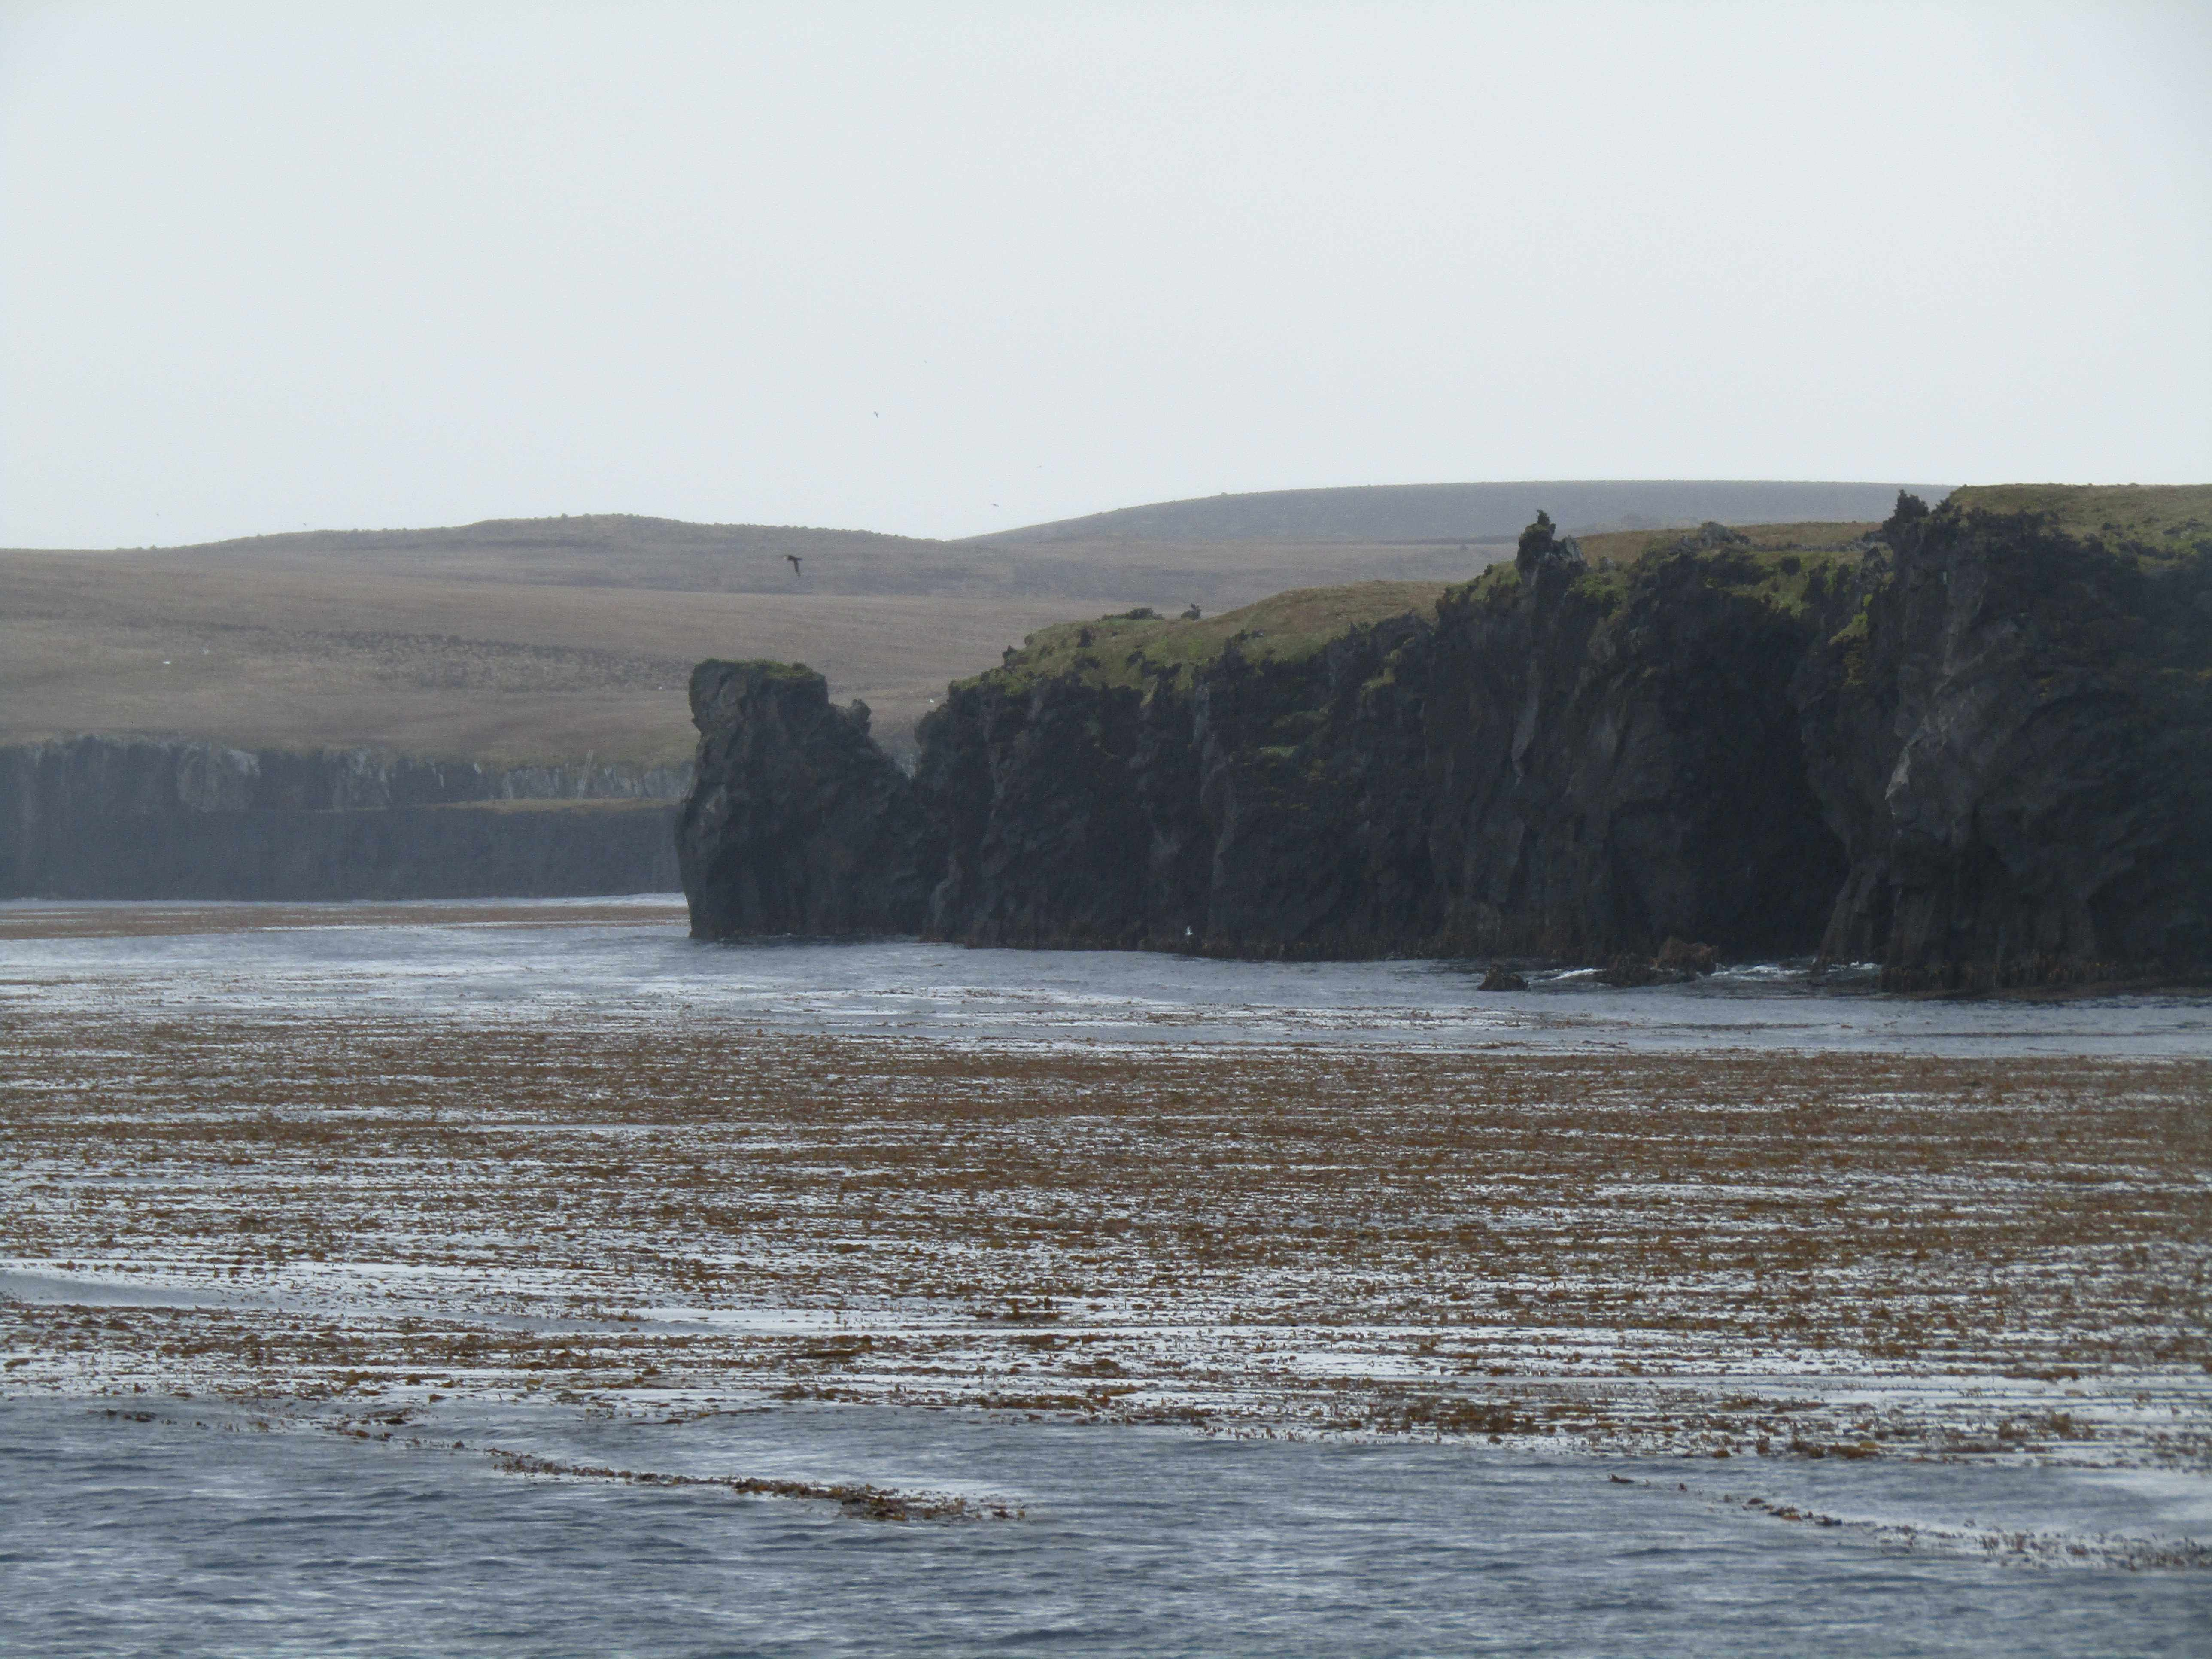
\includegraphics[width=0.7\linewidth]{acantilados_isla_marion.JPG}
\end{figure}
\tiny  Picture: Marion Island. ACE Expedition - Leg 1.
\end{frame}

%----------------------------------------------------------------------------------------

\end{document}